\documentclass[a4paper]{article}

%%%%%%%%%%%%%%%%%%%%%%%%%%%%%%%%%%%%%%%%%%%%%%%%%%%%%%%%%%%%%%%%%%%%%%%%%%%%
% Some common includes. Add additional includes you need.
%%%%%%%%%%%%%%%%%%%%%%%%%%%%%%%%%%%%%%%%%%%%%%%%%%%%%%%%%%%%%%%%%%%%%%%%%%%%
\RequirePackage{ngerman}
\RequirePackage[utf8]{inputenc}
\RequirePackage[T1]{fontenc}
\RequirePackage[margin=30mm,bottom=40mm]{geometry}
\RequirePackage{graphicx}
\RequirePackage{amsmath,amsfonts,amssymb,amsthm}
\RequirePackage{listingsutf8}
\RequirePackage{textcomp}
\RequirePackage{soul}
\RequirePackage{hyperref}
\RequirePackage{tikz}

\renewcommand{\baselinestretch}{1.15} % Line spacing

\usetikzlibrary{arrows.meta}

%%%%%%%%%%%%%%%%%%%%%%%%%%%%%%%%%%%%%%%%%%%%%%%%%%%%%%%%%%%%%%%%%%%%%%%%%%%%
% Defines for mathematical notation. Add additional defines as needed.
%%%%%%%%%%%%%%%%%%%%%%%%%%%%%%%%%%%%%%%%%%%%%%%%%%%%%%%%%%%%%%%%%%%%%%%%%%%%
\def\O{\mathcal{O}}
\def\sort{\mathrm{sort}}
\def\scan{\mathrm{scan}}
\def\dist{\mathrm{dist}}





\newtheorem{theorem}{Satz}


\theoremstyle{definition}
\newtheorem{definition}{Definition}

\theoremstyle{remark}
\newtheorem*{remark}{Bemerkung}

\def\proofname{Beweis}


\usepackage{listings}
\lstset{%
  showstringspaces=false,
  mathescape=true,
  inputencoding=utf8,
  numbers=left,
  xleftmargin=\parindent,
  basicstyle=\footnotesize\ttfamily,
  keywordstyle=\bfseries\color{green!40!black},
  commentstyle=\normalfont\itshape\color{black!60},
  identifierstyle=\color{blue},
  stringstyle=\color{violet},
  tabsize=2%
}


\begin{document}
	\begin{titlepage}
	
	\begin{center}

		\huge \textbf{\textsf{
		\\Arithmetisches Kodieren}} \\
		\LARGE\textbf{\textsc{\\
		Vito Schopper - 7503386
		\\
		Mario Navarro - }}\\ 
		\vspace{2cm}
		\LARGE\textbf{\textsc{\\Pro-Seminar
		\\ Datenkompression WS 2022}}\\ 
		\vspace{2.5cm}
		\large \textbf{
		\\
				Dozent: {Dr.- Ing. The Anh Vuong} \\
Graphische Daten Verarbeitung, Informatik Institut
\\
Goethe Universität , Frankfurt am Main
}
	\end{center}

\end{titlepage}
\tableofcontents\newpage
%\listoffigures\newpage
	
\section{Thema}
\label{sec:Thema}
Arithmetisches Kodieren ist eine Form der Entropiekodierung. Im Gegensatz zu anderen Entropiekodierungen wie z.B. der Huffman-Kodierung, wo ein Baum erstellt wird um anschließend für jedes Zeichen eine individuelle Kodierung zu berechnen, wird beim Arithmetischen Kodieren eine lange binäre Fließkommazahl ausgegeben, welche die komplette Eingabe kodiert. Es findet also keine Kodierung kleinerer Komponente statt, sondern es wird Zeichen für Zeichen kodiert. Hierdurch werden Kompressionsraten erreicht, welche sehr nahe am theoretischen Limit der Entropie liegen.\cite{WIKI}
		\section{Theoretische Grundlagen}

	\newpage
		\section{Verfahren-Beschreibung}
Zunächst wird für die Eingabe die Häufigkeiten aller vorkommenden Zeichen berechnet. Anschließend wird das Interval [0,1] entsprechend dieser Häufigkeiten aufgeteilt. Dies wird gemacht, da am Ende  beim Arithmetischen Kodieren die Eingabe als eine beliebig lange Fließkommazahl kodiert wird. Legen wir nun das Intervall [0,1] fest, so wird der später kodierte String irgendwo zwischen 0 und 1 liegen.
So könnte z.B für die Eingabe \textbf{Hello} folgende Startbedingung erstellt werden.
\\\\
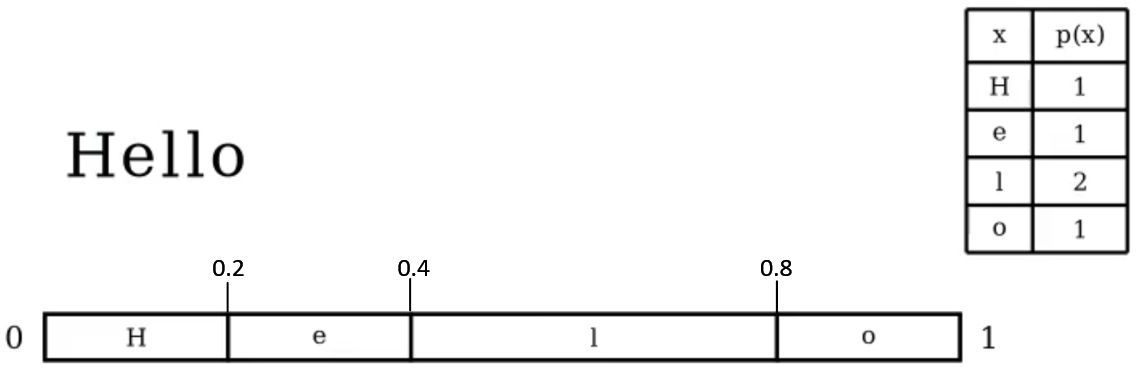
\includegraphics[scale=0.5]{schritt1}
\\\\
Nun wird das erste Zeichen eingelesen. Dessen Intervall wird nun das komplette Intervall ersetzen. Die Verhältnisse der Intervalle untereinander ändert sich nicht. Es werden lediglich die Grenzen aktualisiert.
\\
\begin{center}
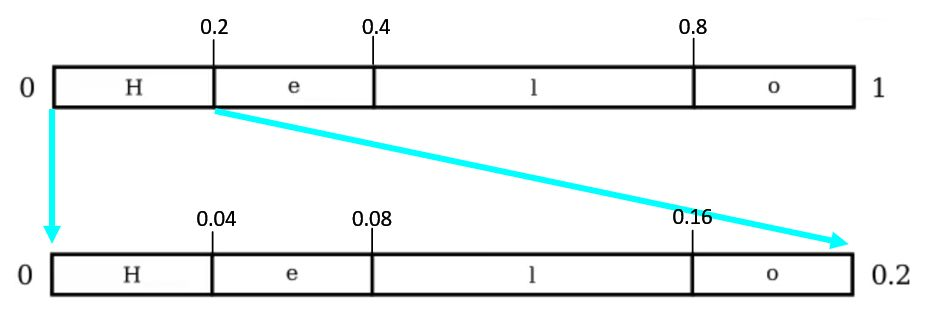
\includegraphics[scale=0.5]{schritt2}
\end{center}
Nun wird das nächste Zeichen eingelesen und die Intervallgrenzen entsprechend aktualisiert. Hat man dies nun für alle Zeichen der Eingabe durchgeführt, so liegt einem ein Intervall [a,b] vor.\\
Alle Zahlen innerhalb dieses Intervalls sind korrekte Kodierungen für unsere Eingabe. Es gibt somit theoretisch unendlich viele Kodierungen für eine Eingabe x, nämlich alle Zahlen im Intervall [a,b].\\
Da man bei einer Kodierung eine Eingabe aber natürlich mit möglichst wenig Bits kodieren möchte, wird die kürzeste Binärzahl genommen, welche im Intervall [a,b] liegt.\\
Angenommen uns liegt am Ende das Intervall [0.78, 0.8] vor
Es wird bei $0.1_2$ gestartet und geprüft, ob diese Zahl schon im Intervall [0.78, 0.8] liegt.\\
Da $0.1_2 = 0.5_{10}$ noch unterhalb des Intervalls liegt, muss unsere Binärzahl erhöht werden.\\
$0.11_2 = 0.75_{10}$ ist schon sehr Nahe an unserem Intervall, jedoch liegt es noch nicht darin.Da zweite Bit ist somit eine 1 und wir erhöhen um 1 Bit.\\
$0.111_2 = 0.875_{10}$ liegt leider drüber, somit ist das dritte Bit eine 0.
\\
$0.1101_2 = 0.8125_{10}$ liegt wieder drüber, somit ist das vierte Bit eine 0.
\\
$0.11001_2 = 0.78125_{10}$ liegt nun endlich vollkommen in unserem Intervall [0.78, 0.8].
\\
0.11001 ist somit die kürzeste Kodierung für unsere Eingabe.
		\section{Anwendungsgebiet}
	Hier könnte ein kurzer Satz zur Einleitung stehen.
	
			\section{Qualitätsbewertung über das Verfahren}
	Hier könnte ein kurzer Satz zur Einleitung stehen.
	
	\newpage
			\section{Präsentation / Demonstration Kit}
Wir haben bei der Visualisierung/der Umsetzung des Demonstrations Kit zwischen 2 Fällen unterschieden. Da es bei den Berechnungen während der Kodierung/Dekodierung zu Schwierigkeiten mit den Intervallgrenzen kommt (siehe Verfahren Beschreibung), haben wir ein \textbf{naives} und ein \textbf{genaues} Kit erstellt.
\\
\\
Das naive Kit erstellt eine gut verständliche, visuelle Animation. Jedoch funktioniert dieses Verfahren nur für relativ kleine Eingaben wie z.B ``Hello'' oder ``Laterne''. Bei größeren Eingaben benötigt die Erstellung der Animation erheblich länger. Da dieses Verfahren auch nicht das TODO umsetzt, kommt es hier bei größeren Eingaben zu den in Kapitel 3 erwähnten Rundungsfehlern. Auf kurzen Eingaben ist jedoch eine korrekte
Kodierung/Dekodierung, sowie eine Erstellung einer visuell ansprechenden Animation kein Problem. 
\\
\\
Hierfür haben wir auf das python-Modul \textbf{manim} zurückgegriffen. Dabei handelt es sich um ein Opensource-Projekt des Youtubers ``3Blue1Brown'', welcher es vor mehreren Jahren geschrieben hat, um visuell ansprechende Animationen ifür den Bereich der Mathematik zu erstellen.
\\
Mittlerweile wird dieses Model jedoch durch die Community erweitert und bietet viele Möglichkeiten Themen aus dem MINT-Bereich visuell darzustellen.
\subsection{naives Verfahren}
\label{sec:manim}
\subsubsection{Installation}
Es wird das python-modul \textbf{manim}, sowie viele kleine weitere module wie z.B. \textbf{ffmpeg} benötigt, welche jedoch automatisch mit \textbf{manim} heruntergeladen werden.\\
Der Installationsvorgang wird unter \href{https://docs.manim.community/en/stable/installation.html}{https://docs.manim.community/en/stable/installation.html}
genauer beschrieben.
\\
\subsubsection{Kodierung}
Für die Kodierung wird die Datei \textbf{encoding.py} mithilfe des Befehls
\begin{lstlisting}[language=bash,
numbers=none]
manim -pql -v critical encoding.py
\end{lstlisting}
im terminal ausgeführt.
\\
Anschließend wird als Eingabe das zu kodierende Wort erfragt. Hier wie oben erwähnt, kein zu langes Wort eingeben.
Daraufhin kann es je nach länge des Wortes 1-2 min dauern, bis die Animation erstellt
wurde, welche sich direkt in einem neuen Fenster öffnet und angeschaut werden kann.
Alternativ wurde die Animation unter
\begin{lstlisting}[language=bash, numbers=none]
.\SeminarDatenkompression-2022\pythno\media\videos%encodin\480p15\Encoding.mp4
\end{lstlisting}
gespeichert.
\subsubsection{Dekodierung}
Für die Dekodierung wird die Datei \textbf{decoding.py} mithilfe des Befehls
\begin{lstlisting}[language=bash,
numbers=none]
manim -pql -v critical decoding.py
\end{lstlisting}
im terminal ausgeführt.
Anschließend wird als Eingabe zuerst die zu dekodierende Binärzahl
erfragt. Daraufhin wird eine Häufigkeitsverteilung der vorkommenden Buchstaben erfragt.
Diese muss im Format eines python-Dictionaries eingegeben werden.
z.B: TODO: ist Reihenfolge egal?
\begin{lstlisting}[language=bash,
numbers=none]
{"H": 1, "e": 1, "l": 2, "o": 1}
{"A": 1, "e": 1, "f": 2}
\end{lstlisting}
Daraufhin kann es je nach länge des Wortes 1-2 min dauern, bis die Animation erstellt
wurde, welche sich direkt in einem neuen Fenster öffnet und angeschaut werden kann.
Alternativ wurde die Animation unter
\begin{lstlisting}[language=bash,
numbers=none]
.\Seminar-Datenkompression-2022\python%\media\videos\decodin\480p15\Decoding.mp4
\end{lstlisting}
gespeichert.

\subsection{genaues Verfahren}
\label{sec:genaues-Verfahren}
Hierfür bitte die html Datei \textbf{Datenkompression.html} unter \textit{./Seminar-Datenkompression-2022/HTML} öffnen. Die erscheinende Seite, implementiert unsere Kodierungen/Dekodierungen gebündelt in einer html. Hier werden jedoch keine Animationen angezeigt. (Verweis auf \ref{sec:manim})
\subsubsection{Kodierung}
Für die Kodierung wird eine Eingabe im Eingabefeld erwartet. Falls gewünscht kann man sich mit dem Button \textbf{Generiere Wahrscheinlichkeiten}, die Wahrscheinlichkeitsverteilung der Eingabe anzeigen lassen.
\\
Um nun eine genaue Kodierung berechnen zu lassen, nach Eingabe ins obere Feld, den Button \textbf{Starte Genaues-Kompressionsverfahren} drücken.
\\
Anschließend wird der kodierte Binärstring im unteren Feld angezeigt.\\

\subsubsection{Dekodierung}
Um den kodierten Binärstring zu dekodieren, sollte man am besten kurz das obere Eingabefeld manuell leeren. Fügt man nun den kodierten Binärstring ins untere Feld ein und drückt auf \textbf{Starte Genaues-Dekompressionsverfahren}, so wird einem die Dekodierung im oberen Feld angezeigt.


\subsection{naive HTML-Kodierung}
Auf der HTML Seite kann man zusätzlich noch einmal das naive Verfahren ausführen lassen. Das Vorgehen ist analog zu \ref{sec:genaues-Verfahren}.\\
\textit{Anmerkung: Die Kodierung weicht leicht von der Kodierung in den Animationen ab, da der Algorithmus anders implementiert wurde.}


	
	
	
% wird am Ende entfernt. Dient nur zur Referenz für gewisse commands

		
		\newpage
	
	\begin{thebibliography}{2}
		\bibitem{mark-nelson} Mark Nelson. (2014, October 19). Data compression with arithmetic coding. Mark Nelson. Retrieved January 12, 2023, from https://marknelson.us/posts/2014/10/19/data-compression-with-arithmetic-coding.html 
		
		\bibitem{WIKI} Wikimedia Foundation. (n.d.). Arithmetisches Kodieren. Wikipedia. Retrieved January 12, 2023, from https://de.wikipedia.org/wiki/Arithmetisches\_Kodieren
	\end{thebibliography}
\end{document}